\section{Business Cycles: Detrending and the RBC Model}

This section has two parts. First, we explain how economists separate a macroeconomic time series into a slow-moving \emph{trend} and a \emph{cyclical} component (linear detrending and the Hodrick--Prescott filter). Second, we build and solve the basic \emph{Real Business Cycle} (RBC) model, whose job is to explain the cyclical component.

%=====================================================================
\subsection{Business cycles and linear detrending \pg{43}}

\paragraph{Setup.}
\begin{itemize}
  \item Time is discrete, $t=1,2,\dots,T$ (e.g.\ quarters or years).
  \item $x_t>0$: an observed macro series in levels (e.g.\ real GDP).
  \item \textbf{Business cycle} = the deviation of a series from its trend. Because real GDP grows over time, we must first remove the trend component; what remains is the cycle that business-cycle models try to explain.
\end{itemize}

\paragraph{Method 1: linear (log-linear) detrending.}
Assume the series is the \emph{product} of a deterministic exponential trend and a cyclical factor:
\begin{equation}\label{eq:s6_lintrend}
x_t=\underbrace{x_0e^{\gamma t}}_{\text{trend}}\cdot\underbrace{\bar x_t}_{\text{cycle}} ,
\end{equation}
where
\begin{itemize}
  \item $x_0>0$ is the trend level at $t=0$;
  \item $\gamma$ is the constant trend growth rate (since $\frac{d}{dt}\ln(x_0e^{\gamma t})=\gamma$);
  \item $\bar x_t>0$ is the cyclical factor: $\bar x_t>1$ means the series is above trend (expansion), $\bar x_t<1$ below trend (contraction), $\bar x_t=1$ exactly on trend.
\end{itemize}
Take natural logs of \eqref{eq:s6_lintrend}, using $\ln(ab)=\ln a+\ln b$ and $\ln e^{\gamma t}=\gamma t$:
\begin{align}
\ln x_t&=\ln x_0+\ln e^{\gamma t}+\ln\bar x_t \notag\\
&=\underbrace{\ln x_0}_{a}+\underbrace{\gamma}_{b}\,t+\underbrace{\ln\bar x_t}_{e_t}. \label{eq:s6_linreg}
\end{align}
This is a linear regression of $\ln x_t$ on a constant and a time trend, $\ln x_t=a+bt+e_t$.
\begin{itemize}
  \item Estimate $a$ and $b$ by OLS: $\hat b=\dfrac{\sum_t(t-\bar t)(\ln x_t-\overline{\ln x})}{\sum_t(t-\bar t)^2}$, $\hat a=\overline{\ln x}-\hat b\,\bar t$ (bars denote sample means).
  \item The cyclical component is the OLS residual: the fitted trend is \emph{subtracted from} the series,
  \[
  \ln\bar x_t=\ln x_t-\hat a-\hat b\,t .
  \]
  Since $\ln\bar x_t\approx\bar x_t-1$ for $\bar x_t$ near 1, the residual is approximately the percentage deviation from trend.
  \item \textbf{Problem:} real series contain a \emph{stochastic} trend (permanent shocks shift the level of GDP for good). A straight line cannot follow such shifts, so part of the permanent component stays in the residual. The resulting ``cycle'' is too persistent: measured cycles last too long.
\end{itemize}

%=====================================================================
\subsection{The Hodrick--Prescott (HP) filter \pg{43--44}}

\paragraph{Setup.}
\begin{itemize}
  \item $y_t$: the \emph{log} of the observed series at date $t$, for $t=1,\dots,T$ (data, taken as given).
  \item $y_t^g$: the trend (``growth'') component at $t$. The whole path $\{y_t^g\}_{t=1}^T$ is the choice variable.
  \item $y_t^c\equiv y_t-y_t^g$: the cyclical component (the part of the data the trend does not explain).
  \item $\mu\ge0$: a bound on how much the trend's growth rate may change; $\lambda\ge0$: the associated Lagrange multiplier, called the \emph{smoothing parameter}.
\end{itemize}
The HP trend is \emph{not} linear: it is allowed to bend slowly, so it also absorbs a slowly moving stochastic growth component that linear detrending misses.

\paragraph{The problem.} Choose the trend path to stay close to the data, subject to the trend being smooth:
\begin{equation}\label{eq:s6_hp}
\min_{\{y_t^g\}_{t=1}^T}\ \sum_{t=1}^T\left(y_t-y_t^g\right)^2
\quad\text{s.t.}\quad
\sum_{t=2}^{T-1}\Big[(y_{t+1}^g-y_t^g)-(y_t^g-y_{t-1}^g)\Big]^2\le\mu .
\end{equation}
\begin{itemize}
  \item $y_{t+1}^g-y_t^g$ is the trend growth rate between $t$ and $t+1$ (a log difference).
  \item $(y_{t+1}^g-y_t^g)-(y_t^g-y_{t-1}^g)=y_{t+1}^g-2y_t^g+y_{t-1}^g$ is the \emph{second difference}: the change in the trend growth rate. A straight line has all second differences equal to zero.
  \item In words: minimize the sum of squared deviations of the trend from the data, subject to the sum of squared second differences (how much trend growth changes) not being too large.
\end{itemize}

\paragraph{Lagrangian.}
\begin{equation}\label{eq:s6_hpL}
\mathcal L=\underbrace{\sum_{t=1}^{T}(y_t-y_t^g)^2}_{\text{(i) fit}}
+\underbrace{\lambda\Big[\sum_{t=2}^{T-1}\big(y_{t+1}^g-2y_t^g+y_{t-1}^g\big)^2-\mu\Big]}_{\text{(ii) smoothness}} .
\end{equation}
\begin{itemize}
  \item Think of $\mathcal L$ as a score that we want to make as small as possible.
  \item Term (i) penalizes the trend for deviating from the data.
  \item Term (ii) penalizes the trend for deviating from a straight line (for changing its growth rate). The weight on this penalty is $\lambda$.
  \item The constant $-\lambda\mu$ does not depend on $\{y_t^g\}$, so for a given $\lambda$ the problem is equivalent to the familiar penalized form
  \[
  \min_{\{y_t^g\}}\ \sum_{t=1}^{T}(y_t-y_t^g)^2+\lambda\sum_{t=2}^{T-1}\big(y_{t+1}^g-2y_t^g+y_{t-1}^g\big)^2 .
  \]
  In practice one picks $\lambda$ directly instead of $\mu$ (a larger $\lambda$ corresponds to a tighter bound $\mu$).
\end{itemize}

\paragraph{First-order condition.} To keep notation light write $g_t\equiv y_t^g$ and $D_s\equiv g_{s+1}-2g_s+g_{s-1}$ for $s=2,\dots,T-1$. Take an interior date $3\le t\le T-2$. The variable $g_t$ appears in the fit term $(y_t-g_t)^2$ and in exactly three second differences:
\begin{align*}
D_{t-1}&=g_t-2g_{t-1}+g_{t-2} &&(\text{coefficient on }g_t:\ +1),\\
D_t&=g_{t+1}-2g_t+g_{t-1} &&(\text{coefficient on }g_t:\ -2),\\
D_{t+1}&=g_{t+2}-2g_{t+1}+g_t &&(\text{coefficient on }g_t:\ +1).
\end{align*}
Differentiate the penalized objective with respect to $g_t$ (chain rule: $\frac{\partial}{\partial g}(f(g))^2=2f(g)f'(g)$) and set to zero:
\begin{align*}
0&=-2(y_t-g_t)+2\lambda\big[D_{t-1}\cdot 1+D_t\cdot(-2)+D_{t+1}\cdot 1\big]\\
\text{Divide by 2:}\quad y_t-g_t&=\lambda\big[D_{t-1}-2D_t+D_{t+1}\big]\\
\text{Expand:}\quad y_t-g_t&=\lambda\big[(g_t-2g_{t-1}+g_{t-2})-2(g_{t+1}-2g_t+g_{t-1})+(g_{t+2}-2g_{t+1}+g_t)\big]\\
\text{Collect terms:}\quad y_t-g_t&=\lambda\big[g_{t-2}-4g_{t-1}+6g_t-4g_{t+1}+g_{t+2}\big].
\end{align*}
\begin{keybox}[title=HP filter first-order condition]
For interior dates,
\[
y_t^c=y_t-y_t^g=\lambda\big(y_{t-2}^g-4y_{t-1}^g+6y_t^g-4y_{t+1}^g+y_{t+2}^g\big),
\]
i.e.\ the cycle equals $\lambda$ times the fourth difference of the trend. At the ends the pattern is truncated, e.g.\ $y_1-y_1^g=\lambda(y_1^g-2y_2^g+y_3^g)$ and $y_2-y_2^g=\lambda(-2y_1^g+5y_2^g-4y_3^g+y_4^g)$. Stacking all $T$ conditions: $(I+\lambda K'K)\,y^g=y$, where $K$ is the $(T-2)\times T$ second-difference matrix, so $y^g=(I+\lambda K'K)^{-1}y$ is a linear filter of the data.
\end{keybox}
Interpretation: at the optimum, the marginal gain from moving the trend closer to the data (left side) equals the marginal cost in lost smoothness (right side). Because $K$ maps any constant or linear sequence to zero, summing the FOCs gives $\sum_t y_t^c=0$: the cycle averages to zero.

\paragraph{Role of the smoothing parameter $\lambda$.}
\begin{itemize}
  \item $\lambda=0$: no smoothness penalty, so the best fit is $y_t^g=y_t$ for all $t$. The trend equals the data and there is no cycle.
  \item $\lambda\to\infty$: any nonzero second difference becomes infinitely costly, so $(y_{t+1}^g-y_t^g)-(y_t^g-y_{t-1}^g)=0$ for all $t$. Constant growth means $y^g$ is a \textbf{linear trend}, and the HP filter collapses to Method 1.
  \item In between, a larger $\lambda$ gives a smoother trend and a larger, more persistent cycle.
\end{itemize}
\begin{keybox}[title=Standard values of $\lambda$]
Quarterly data: $\lambda=1600$. \quad Annual data: $\lambda=100$ (conventional) or $\lambda=6.25$ (Ravn--Uhlig). \quad Monthly data: $\lambda=14400$.\\[2pt]
The Ravn--Uhlig rule rescales by the fourth power of the observation-frequency ratio: $1600/4^4=6.25$ for annual data.
\end{keybox}

%=====================================================================
\subsection{The RBC model: setup \pg{62}}

\begin{keybox}[title=RBC model]
RBC model $=$ neoclassical growth model $+$ endogenous labour/leisure choice $+$ random technology (TFP) shocks.
\end{keybox}

\paragraph{Setup (variables and parameters).} Time is discrete, $t=0,1,2,\dots$; there is no population or trend growth.
\begin{itemize}
  \item $y_t$: output; $c_t$: consumption; $i_t$: investment; $k_t$: capital stock at the start of period $t$ (chosen at $t-1$, so it is \emph{predetermined} at $t$).
  \item $l_t\in[0,1]$: hours worked. The time endowment is normalized to 1, so leisure is $1-l_t$.
  \item $A_t$: total factor productivity (labour-augmenting technology), random.
  \item $w_t$: real wage; $r_t$: real interest rate, \emph{net} of depreciation. The rental price of capital is $r_t+\delta$.
  \item $\alpha\in(0,1)$: capital share; $\delta\in(0,1]$: depreciation rate; $\beta\in(0,1)$: discount factor; $b>0$: weight on leisure; $\rho_A$: persistence of TFP; $\sigma_A$: standard deviation of TFP shocks.
\end{itemize}

\paragraph{Production and goods market.} A Cobb--Douglas technology with constant returns to scale:
\begin{equation}\label{eq:s6_prod}
y_t=k_t^{\alpha}(A_tl_t)^{1-\alpha},\qquad y_t=c_t+i_t .
\end{equation}

\paragraph{Capital accumulation.} Capital depreciates at rate $\delta$ and is replenished by investment; substituting $i_t=y_t-c_t$:
\begin{equation}\label{eq:s6_kacc}
k_{t+1}=(1-\delta)k_t+i_t=(1-\delta)k_t+y_t-c_t .
\end{equation}

\paragraph{Household preferences.} An infinitely lived representative household maximizes
\begin{equation}\label{eq:s6_U}
U=E_0\sum_{t=0}^\infty\beta^t u(c_t,1-l_t),\qquad u(c_t,1-l_t)=\ln c_t+b\ln(1-l_t).
\end{equation}
\begin{itemize}
  \item $\beta^t$ discounts utility in period $t$ back to period $0$; $\beta\to1$ means the household values the future more.
  \item A larger $b$ means leisure is more important relative to consumption.
  \item $E_0$ is the expectation conditional on information at $t=0$: the household faces uncertainty about future TFP, so it maximizes \emph{expected} utility. More generally $E_t$ denotes expectation given information at $t$ (which includes $A_t$ and $k_t$).
\end{itemize}

\paragraph{Technology process.} Log TFP follows an AR(1):
\begin{equation}\label{eq:s6_ar1}
\ln A_t=\rho_A\ln A_{t-1}+\varepsilon_{A,t},\qquad -1<\rho_A<1,\qquad \varepsilon_{A,t}\sim\text{i.i.d. }N(0,\sigma_A^2).
\end{equation}
\begin{itemize}
  \item $\rho_A$ measures persistence: after a shock $\varepsilon_{A,t}$, $\ln A_{t+j}$ is affected by $\rho_A^{\,j}\varepsilon_{A,t}$.
  \item $|\rho_A|<1$ makes the process stationary: shocks do not explode and eventually die out, and the unconditional mean of $\ln A_t$ is $0$ (so $A=1$ on average).
  \item $\rho_A=0$: TFP is a pure i.i.d.\ shock with no memory. $\rho_A=1$: random walk, every shock is permanent.
\end{itemize}

%=====================================================================
\subsection{Firm's problem \pg{62}}

A representative firm rents capital and hires labour in competitive markets, taking $w_t$ and $r_t$ as given. Each period it solves
\[
\max_{k_t,l_t}\ \pi_t=k_t^{\alpha}(A_tl_t)^{1-\alpha}-w_tl_t-(r_t+\delta)k_t .
\]
\textbf{FOC for labour.} Differentiate with respect to $l_t$ (power rule; $(A_tl_t)^{1-\alpha}=A_t^{1-\alpha}l_t^{1-\alpha}$):
\begin{align*}
0&=(1-\alpha)k_t^{\alpha}A_t^{1-\alpha}l_t^{-\alpha}-w_t\\
\Rightarrow\ w_t&=(1-\alpha)k_t^{\alpha}(A_tl_t)^{-\alpha}A_t \quad\text{(regroup }A_t^{1-\alpha}l_t^{-\alpha}=(A_tl_t)^{-\alpha}A_t)\\
&=(1-\alpha)\Big(\frac{k_t}{A_tl_t}\Big)^{\alpha}A_t\\
&=(1-\alpha)\frac{y_t}{l_t}\quad\text{(multiply and divide by }l_t\text{ and use \eqref{eq:s6_prod})}.
\end{align*}
\textbf{FOC for capital.} Differentiate with respect to $k_t$:
\begin{align*}
0&=\alpha k_t^{\alpha-1}(A_tl_t)^{1-\alpha}-(r_t+\delta)\\
\Rightarrow\ r_t+\delta&=\alpha\Big(\frac{A_tl_t}{k_t}\Big)^{1-\alpha}=\alpha\frac{y_t}{k_t}
\quad\text{(since }k_t^{\alpha-1}=k_t^{\alpha}/k_t).
\end{align*}
\begin{keybox}[title=Factor prices]
\begin{equation}\label{eq:s6_prices}
w_t=MPL_t=(1-\alpha)\Big(\frac{k_t}{A_tl_t}\Big)^{\alpha}A_t=(1-\alpha)\frac{y_t}{l_t},
\qquad
r_t=MPK_t-\delta=\alpha\Big(\frac{A_tl_t}{k_t}\Big)^{1-\alpha}-\delta=\alpha\frac{y_t}{k_t}-\delta .
\end{equation}
\end{keybox}
\begin{itemize}
  \item Factors are paid their marginal products. With constant returns, $w_tl_t+(r_t+\delta)k_t=(1-\alpha)y_t+\alpha y_t=y_t$, so profits are zero (Euler's theorem for homogeneous functions).
  \item The firm's problem is \textbf{static} (no dynamic programming): it rents $k_t$ freely each period instead of owning it, and takes prices as given, so nothing it does today affects its future options. It simply maximizes current profit.
  \item The household's problem is \textbf{dynamic}, with two margins: \emph{intertemporal} (consume today vs.\ save in capital, because $k$ carries over) and \emph{intratemporal} (work vs.\ leisure within a period).
\end{itemize}

%=====================================================================
\subsection{Household optimality conditions \pg{63}}

\paragraph{Household budget constraint.} The household owns the capital stock, rents it to the firm at $r_t+\delta$, loses $\delta k_t$ to depreciation, earns $w_tl_t$, and consumes $c_t$. Next period's capital is therefore
\begin{align}
k_{t+1}&=(1-\delta)k_t+(r_t+\delta)k_t+w_tl_t-c_t\notag\\
&=(1+r_t)k_t+w_tl_t-c_t . \label{eq:s6_hhbc}
\end{align}
(Using $w_tl_t+(r_t+\delta)k_t=y_t$ turns \eqref{eq:s6_hhbc} back into the resource constraint \eqref{eq:s6_kacc}.)

\paragraph{(1) Intuitive (perturbation) approach.} At an optimum, a small feasible change in the plan cannot raise utility, so marginal cost $=$ marginal benefit.

\emph{Consume or save?} Cut consumption at $t$ by a small $\Delta c$ and save it.
\begin{itemize}
  \item Cost today: utility falls by $\beta^t\,u_c(t)\,\Delta c=\beta^t\frac{1}{c_t}\Delta c$ (since $\partial\ln c/\partial c=1/c$).
  \item Benefit tomorrow: the saving returns $(1+r_{t+1})\Delta c$ of extra consumption at $t+1$, worth $\beta^{t+1}\frac{1+r_{t+1}}{c_{t+1}}\Delta c$; as $r_{t+1},c_{t+1}$ are not known at $t$, take $E_t$.
\end{itemize}
Setting cost $=$ expected benefit and dividing by $\beta^t\Delta c$:
\begin{align}
\beta^t\frac{1}{c_t}\Delta c&=\beta^{t+1}E_t\Big[\frac{1+r_{t+1}}{c_{t+1}}\Big]\Delta c\notag\\
\Rightarrow\quad \frac1{c_t}&=\beta E_t\Big[\frac{1+r_{t+1}}{c_{t+1}}\Big]\qquad\text{(consumption Euler equation).}\label{eq:s6_euler}
\end{align}

\emph{Work or leisure?} Work a little more, $\Delta l$, at date $t$.
\begin{itemize}
  \item Cost: leisure falls by $\Delta l$; utility falls by $\beta^t\frac{b}{1-l_t}\Delta l$ (chain rule: $\frac{\partial}{\partial l}b\ln(1-l)=-\frac{b}{1-l}$).
  \item Benefit: extra earnings $w_t\Delta l$ are consumed, raising utility by $\beta^t\frac{1}{c_t}w_t\Delta l$.
\end{itemize}
Setting them equal and dividing by $\beta^t\Delta l$:
\begin{equation}\label{eq:s6_labour}
\frac{b}{1-l_t}=\frac{w_t}{c_t}\quad\Longleftrightarrow\quad w_t=\frac{b\,c_t}{1-l_t}\qquad\text{(intratemporal labour-supply condition).}
\end{equation}
Interpretation: the real wage equals the marginal rate of substitution between leisure and consumption, $u_{1-l}/u_c=\frac{b/(1-l_t)}{1/c_t}$.

\paragraph{(2) Lagrangian approach.} The household solves
\[
\max_{\{c_t,l_t,k_{t+1}\}_{t\ge0}}E_0\sum_{t=0}^\infty\beta^t\big[\ln c_t+b\ln(1-l_t)\big]\quad\text{s.t. \eqref{eq:s6_hhbc} for every }t,
\]
given $k_0$ and taking $\{w_t,r_t\}$ as given. Attach a (current-value) multiplier $\lambda_t$ to each period's constraint, inside the discounted sum:
\[
\mathcal L=E_0\sum_{t=0}^\infty\beta^t\Big\{\ln c_t+b\ln(1-l_t)+\lambda_t\big[(1+r_t)k_t+w_tl_t-c_t-k_{t+1}\big]\Big\}.
\]
$\lambda_t$ is the marginal utility of one extra unit of goods (wealth) at date $t$.

Differentiate term by term (the derivative of an expectation is the expectation of the derivative):
\begin{itemize}
  \item $[c_t]$: $c_t$ appears only in period $t$: $\beta^t\big(\frac1{c_t}-\lambda_t\big)=0\ \Rightarrow\ \dfrac1{c_t}=\lambda_t$.
  \item $[l_t]$: chain rule on $\ln(1-l_t)$: $\beta^t\big(-\frac{b}{1-l_t}+\lambda_tw_t\big)=0\ \Rightarrow\ \dfrac{b}{1-l_t}=w_t\lambda_t$.
  \item $[k_{t+1}]$: $k_{t+1}$ appears in period $t$'s constraint (as $-k_{t+1}$) and in period $t+1$'s constraint (as $(1+r_{t+1})k_{t+1}$):
  \[
  -\beta^t\lambda_t+\beta^{t+1}E_t\big[\lambda_{t+1}(1+r_{t+1})\big]=0\ \Rightarrow\ \lambda_t=\beta E_t\big[(1+r_{t+1})\lambda_{t+1}\big].
  \]
\end{itemize}
Eliminate $\lambda$: substitute $\lambda_t=1/c_t$ and $\lambda_{t+1}=1/c_{t+1}$ into $[k_{t+1}]$ to get \eqref{eq:s6_euler}; substitute $\lambda_t=1/c_t$ into $[l_t]$ to get \eqref{eq:s6_labour}. The same answers as the intuitive approach.

The \textbf{transversality condition} (TVC) completes the optimality conditions: $\lim_{T\to\infty}\beta^TE_0[\lambda_Tk_{T+1}]=0$, i.e.\ the household does not accumulate capital whose discounted value never gets consumed.

\paragraph{(3) Bellman (dynamic programming) view.} Equivalently, with value function $V(k_t,A_t)$,
\[
V(k_t,A_t)=\max_{c_t,l_t,k_{t+1}}\big\{\ln c_t+b\ln(1-l_t)+\beta E_tV(k_{t+1},A_{t+1})\big\}\ \ \text{s.t. \eqref{eq:s6_hhbc}}.
\]
The FOC for $k_{t+1}$ (after substituting $c_t$ from the constraint) is $\frac1{c_t}=\beta E_t[V_k(k_{t+1},A_{t+1})]$, and the \emph{envelope theorem} (the derivative of the value function w.r.t.\ a state equals the partial derivative of the objective, holding choices fixed) gives $V_k(k_t,A_t)=\frac{1+r_t}{c_t}$. Combining the two yields \eqref{eq:s6_euler} again.

\begin{keybox}[title=Two household optimality conditions]
\[
\frac1{c_t}=\beta E_t\Big[\frac{1+r_{t+1}}{c_{t+1}}\Big]\quad\text{(intertemporal)},\qquad\qquad w_t=\frac{b\,c_t}{1-l_t}\quad\text{(intratemporal)}.
\]
\end{keybox}

%=====================================================================
\subsection{Special case: full depreciation ($\delta=1$), closed form \pg{64}}

With $\delta=1$, capital lasts one period and \eqref{eq:s6_kacc} becomes $k_{t+1}=i_t=y_t-c_t$. Also, from \eqref{eq:s6_prices}, $1+r_{t+1}=\alpha\frac{y_{t+1}}{k_{t+1}}-1+1=\alpha\frac{y_{t+1}}{k_{t+1}}$.

\paragraph{Guess.} There is a constant saving rate $s$ (to be verified):
\[
c_t=(1-s)y_t,\qquad k_{t+1}=i_t=s\,y_t .
\]
The strategy (guess and verify): use the labour condition to show $l_t$ is constant if $s$ is constant, then use the Euler equation to show the guess is consistent with a constant $s$ and find its value.

\paragraph{Step 1: labour condition $\Rightarrow$ constant hours.} Combine the firm's wage $w_t=(1-\alpha)y_t/l_t$ from \eqref{eq:s6_prices} with \eqref{eq:s6_labour}:
\begin{align*}
(1-\alpha)\frac{y_t}{l_t}&=\frac{b\,c_t}{1-l_t}\\
\text{Substitute }c_t=(1-s)y_t:\quad (1-\alpha)\frac{y_t}{l_t}&=\frac{b(1-s)y_t}{1-l_t}\\
\text{Divide by }(1-s)y_t\text{, multiply by }l_t:\quad \frac{1-\alpha}{1-s}&=\frac{b\,l_t}{1-l_t}.
\end{align*}
The left side is a constant if $s$ is constant, so $l_t/(1-l_t)$, and hence $l_t$, is constant: $l_t=l$ for all $t$.

\paragraph{Step 2: Euler equation $\Rightarrow$ $s$ is constant and equals $\alpha\beta$.}
\begin{align*}
\frac1{c_t}&=\beta E_t\Big[\frac{1+r_{t+1}}{c_{t+1}}\Big]\\
\text{Substitute the guess and }1+r_{t+1}=\alpha\tfrac{y_{t+1}}{k_{t+1}}:\quad
\frac1{(1-s)y_t}&=\beta E_t\Big[\frac{\alpha\,y_{t+1}/k_{t+1}}{(1-s)y_{t+1}}\Big]\\
\text{Cancel }y_{t+1}\text{ inside the expectation:}\quad
\frac1{(1-s)y_t}&=\beta E_t\Big[\frac{\alpha}{(1-s)k_{t+1}}\Big]\\
\text{Substitute }k_{t+1}=sy_t:\quad
\frac1{(1-s)y_t}&=\beta E_t\Big[\frac{\alpha}{(1-s)s\,y_t}\Big]\\
y_t\text{ is known at }t\text{, so }E_t\text{ drops:}\quad
\frac1{(1-s)y_t}&=\frac{\alpha\beta}{(1-s)s\,y_t}\\
\text{Multiply both sides by }(1-s)s\,y_t:\quad s&=\alpha\beta .
\end{align*}
The random $y_{t+1}$ cancels \emph{before} taking expectations; this is why the guess works despite uncertainty. Since $s=\alpha\beta$ is a constant, the guess is verified.

\paragraph{Step 3: solve for hours.} Plug $s=\alpha\beta$ into Step 1 and solve for $l$:
\begin{align*}
\frac{1-\alpha}{1-\alpha\beta}&=\frac{b\,l}{1-l}\\
\text{Cross-multiply:}\quad (1-\alpha)(1-l)&=b(1-\alpha\beta)\,l\\
\text{Collect }l:\quad (1-\alpha)&=l\big[(1-\alpha)+b(1-\alpha\beta)\big]\\
\Rightarrow\quad l&=\frac{1-\alpha}{(1-\alpha)+b(1-\alpha\beta)} .
\end{align*}

\begin{keybox}[title={$\delta=1$ closed-form solution}]
\[
s=\alpha\beta,\qquad c_t=(1-\alpha\beta)y_t,\qquad k_{t+1}=\alpha\beta\,y_t,\qquad
l_t=l=\frac{1-\alpha}{(1-\alpha)+b(1-\alpha\beta)},\qquad w_t=\frac{b(1-\alpha\beta)}{1-l}\,y_t .
\]
\end{keybox}
Interpretation: the household always saves the fraction $\alpha\beta$ of output and works a fixed number of hours, regardless of the TFP shock. More patience ($\beta\uparrow$) or a more productive capital ($\alpha\uparrow$) raises saving; a stronger taste for leisure ($b\uparrow$) lowers hours ($\partial l/\partial b<0$ because $b$ appears only in the denominator).

\begin{tipbox}
Why do hours not respond to TFP? A positive TFP shock raises the wage. \emph{Substitution effect:} leisure is now more expensive, so work more. \emph{Income (wealth) effect:} the household is richer, so it consumes more of everything, including leisure, and works less. With $\ln c+b\ln(1-l)$ utility and $\delta=1$, consumption rises one-for-one in percent with the wage, and the two effects exactly cancel.
\end{tipbox}

%=====================================================================
\subsection{The $\delta=1$ case: successes, failures, and propagation \pg{64--65}}

\paragraph{Successes.}
\begin{itemize}
  \item Output, consumption, investment and next period's capital are all procyclical: $c_t=(1-s)y_t$, $i_t=k_{t+1}=s\,y_t$ move with $y_t$.
  \item Consumption is less volatile than output in levels: $\mathrm{var}(c_t)=(1-s)^2\mathrm{var}(y_t)<\mathrm{var}(y_t)$.
\end{itemize}

\paragraph{Failures.}
\begin{enumerate}
  \item \textbf{Zero variation in hours}: $l_t=l$, while hours are strongly procyclical in the data.
  \item \textbf{Investment too smooth}: $\mathrm{var}(i_t)=\mathrm{var}(sy_t)=s^2\mathrm{var}(y_t)<\mathrm{var}(y_t)$. In the data $\mathrm{var}(c)<\mathrm{var}(y)<\mathrm{var}(i)$. (In logs, $\ln c_t=\ln(1-s)+\ln y_t$ and $\ln i_t=\ln s+\ln y_t$, so in percentage terms $c$, $i$, $y$ are \emph{equally} volatile, also counterfactual.)
  \item \textbf{Wages too procyclical}: substituting $c_t=(1-s)y_t$ into \eqref{eq:s6_labour} gives $w_t=\frac{b(1-s)}{1-l}\,y_t$, proportional to output. In the data wages are only mildly procyclical (wage rigidity).
  \item \textbf{Weak propagation}: technology shocks have only temporary effects on output beyond the persistence of $A_t$ itself. With $\delta=1$, capital is used up every period, so there is no slowly decaying capital stock to carry the shock forward.
\end{enumerate}

\paragraph{Output dynamics with $\delta=1$: an AR(2).} Let $\tilde y_t\equiv\ln y_t-E[\ln y_t]$ and $a_t\equiv\ln A_t$.
\begin{align*}
\ln y_t&=\alpha\ln k_t+(1-\alpha)\ln A_t+(1-\alpha)\ln l &&\text{(log of \eqref{eq:s6_prod})}\\
&=\alpha\big(\ln s+\ln y_{t-1}\big)+(1-\alpha)a_t+(1-\alpha)\ln l &&\text{(substitute }k_t=sy_{t-1})\\
\Rightarrow\ \tilde y_t&=\alpha\tilde y_{t-1}+(1-\alpha)a_t &&\text{(subtract the mean; constants drop).}
\end{align*}
Now remove $a_t$ using the AR(1) \eqref{eq:s6_ar1}. Write the last line at $t-1$ and multiply by $\rho_A$: $\rho_A\tilde y_{t-1}=\alpha\rho_A\tilde y_{t-2}+(1-\alpha)\rho_Aa_{t-1}$. Subtract this from the line at $t$:
\begin{align*}
\tilde y_t-\rho_A\tilde y_{t-1}&=\alpha\tilde y_{t-1}-\alpha\rho_A\tilde y_{t-2}+(1-\alpha)(a_t-\rho_Aa_{t-1})\\
\Rightarrow\ \tilde y_t&=(\alpha+\rho_A)\tilde y_{t-1}-\alpha\rho_A\tilde y_{t-2}+(1-\alpha)\varepsilon_{A,t}.
\end{align*}
\begin{keybox}[title={Output is AR(2) when $\delta=1$}]
\[
\tilde y_t=(\alpha+\rho_A)\tilde y_{t-1}-\alpha\rho_A\tilde y_{t-2}+(1-\alpha)\varepsilon_{A,t}.
\]
\end{keybox}
Interpretation: the two roots are $\rho_A$ (TFP persistence) and $\alpha$ (capital carries part of today's output into tomorrow). The impulse response is $(1-\alpha)$ on impact and $(1-\alpha)(\alpha+\rho_A)$ one period later, so it is \emph{hump-shaped} if $\alpha+\rho_A>1$. But with $\alpha\approx1/3$ the capital channel adds little: output persistence is essentially that of $A_t$.

\begin{center}
\renewcommand{\arraystretch}{1.15}
\begin{tabular}{p{2.2cm}p{6cm}p{6cm}}
\hline
 & General case ($\delta<1$) & Special case ($\delta=1$)\\\hline
TFP & AR(1) & AR(1)\\
Capital & accumulates smoothly; a shock propagates for a long time & fully depreciates each period; a shock's effect is short-lived\\
Hours $l_t$ & endogenous, time-varying & constant\\
Output IRF & jumps on impact, long tail & hump shape, dies out quickly\\\hline
\end{tabular}
\end{center}

\begin{center}
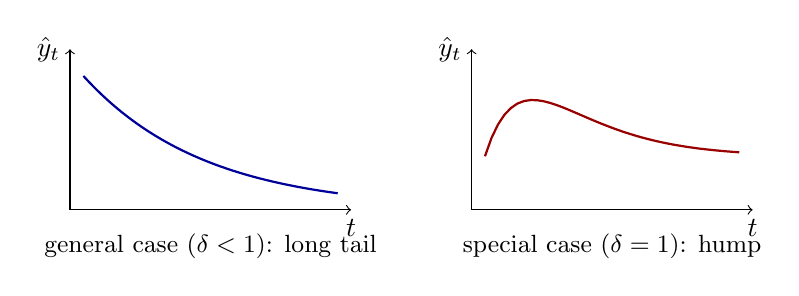
\begin{tikzpicture}[scale=0.85]
  \draw[->] (0,0)--(4.2,0) node[below]{$t$}; \draw[->] (0,0)--(0,2.4) node[left]{$\hat y_t$};
  \draw[thick,blue!60!black,domain=0.2:4,samples=40] plot(\x,{2*exp(-0.55*(\x-0.2))});
  \node at (2.1,-0.55){\small general case ($\delta<1$): long tail};
  \begin{scope}[xshift=6cm]
  \draw[->] (0,0)--(4.2,0) node[below]{$t$}; \draw[->] (0,0)--(0,2.4) node[left]{$\hat y_t$};
  \draw[thick,red!60!black,domain=0.2:4,samples=40] plot(\x,{0.8+3.2*(\x-0.2)*exp(-1.4*(\x-0.2))});
  \node at (2.1,-0.55){\small special case ($\delta=1$): hump};
  \end{scope}
\end{tikzpicture}
\end{center}
How to read the figure: each panel plots the response of (log) output to a one-time positive TFP shock, with time on the horizontal axis. In the general case output jumps on impact and then decays slowly, because the extra capital built during the boom wears out only gradually. In the $\delta=1$ case the AR(2) dynamics can produce a small hump, but the response dies out quickly because no capital survives from one period to the next.

\paragraph{Two solution methods.}
\begin{itemize}
  \item \textbf{Planner:} choose quantities directly to maximize welfare subject to the aggregate resource constraint, then recover prices from marginal products. No $w_t,r_t$ appear:
  \[
  \max_{\{c_t,l_t,k_{t+1}\}}E_0\sum_{t=0}^\infty\beta^t\big(\ln c_t+b\ln(1-l_t)\big)\quad\text{s.t.}\quad c_t+k_{t+1}=k_t^\alpha(A_tl_t)^{1-\alpha}+(1-\delta)k_t .
  \]
  \item \textbf{Decentralized:} given prices, solve the household and firm problems subject to their own constraints, then impose market clearing (which pins down prices).
  \item In the RBC model the two methods differ only in the constraint used (aggregate resource constraint vs.\ household budget constraint); there are no distortions, so by the welfare theorems they give the same allocation.
\end{itemize}

%=====================================================================
\subsection{General model ($\delta<1$): equilibrium system \pg{65}}

With $\delta<1$ there is no closed-form solution, so we (i) collect the equilibrium conditions, (ii) find the non-stochastic steady state, (iii) log-linearize around it, and (iv) solve the linear system.

\paragraph{Equilibrium.} Combine the resource constraint \eqref{eq:s6_kacc} with \eqref{eq:s6_prod}, the Euler equation \eqref{eq:s6_euler}, the interest rate from \eqref{eq:s6_prices}, and the labour condition \eqref{eq:s6_labour} with the firm's wage:
\begin{keybox}[title={Equilibrium system (unknowns $c_t,k_{t+1},l_t,r_t$; given $k_t$ and $A_t$)}]
\begin{align}
&c_t+k_{t+1}=(1-\delta)k_t+k_t^{\alpha}(A_tl_t)^{1-\alpha} \label{eq:s6_E1}\\
&\frac1{c_t}=\beta E_t\Big[\frac{1+r_{t+1}}{c_{t+1}}\Big]\label{eq:s6_E2}\\
&r_t=\alpha\Big(\frac{A_tl_t}{k_t}\Big)^{1-\alpha}-\delta\label{eq:s6_E3}\\
&(1-\alpha)\Big(\frac{k_t}{A_tl_t}\Big)^{\alpha}A_t=\frac{b\,c_t}{1-l_t}\label{eq:s6_E4}
\end{align}
plus the TFP process $\ln A_t=\rho_A\ln A_{t-1}+\varepsilon_{A,t}$ and the TVC.
\end{keybox}
Equation \eqref{eq:s6_E4} sets the wage paid by the firm equal to the wage required by the household ($w_t$ has been substituted out).

%=====================================================================
\subsection{Steady state \pg{66}}

In the non-stochastic steady state all shocks are zero, so $\ln A^*=0$, i.e.\ $A^*=1$, and every variable is constant: $x_t=x_{t+1}=x^*$. There is no uncertainty, so the expectation operator disappears. Equations \eqref{eq:s6_E1}--\eqref{eq:s6_E4} become
\begin{align*}
&\text{(a)}\quad c^*+k^*=k^{*\alpha}(A^*l^*)^{1-\alpha}+(1-\delta)k^*,\\
&\text{(b)}\quad \frac1{c^*}=\beta\frac{1+r^*}{c^*},\\
&\text{(c)}\quad r^*=\alpha\Big(\frac{A^*l^*}{k^*}\Big)^{1-\alpha}-\delta,\\
&\text{(d)}\quad w^*=\frac{b\,c^*}{1-l^*}=(1-\alpha)\Big(\frac{k^*}{A^*l^*}\Big)^{\alpha}A^*.
\end{align*}
Solve them in order, setting $A^*=1$.

\textbf{Step 1 (interest rate) from (b).} Multiply both sides by $c^*$:
\[
1=\beta(1+r^*)\quad\Rightarrow\quad r^*=\frac1\beta-1 .
\]
The steady-state interest rate is pinned down by impatience alone.

\textbf{Step 2 (capital--labour ratio) from (c).}
\begin{align*}
r^*+\delta&=\alpha\Big(\frac{l^*}{k^*}\Big)^{1-\alpha}\\
\Rightarrow\ \Big(\frac{k^*}{l^*}\Big)^{1-\alpha}&=\frac{\alpha}{r^*+\delta}\quad\text{(invert both sides)}\\
\Rightarrow\ \frac{k^*}{l^*}&=\Big(\frac{\alpha}{r^*+\delta}\Big)^{\frac1{1-\alpha}}.
\end{align*}

\textbf{Step 3 (ratios and wage).} With $y^*=k^{*\alpha}l^{*1-\alpha}$:
\begin{align*}
\frac{y^*}{k^*}&=\Big(\frac{k^*}{l^*}\Big)^{\alpha-1}=\frac{r^*+\delta}{\alpha}\quad\text{(from Step 2)},\\
w^*&=(1-\alpha)\Big(\frac{k^*}{l^*}\Big)^{\alpha}\quad\text{(from (d))}.
\end{align*}
From (a), the $k^*$ terms give $c^*=y^*-\delta k^*$ (investment just replaces depreciation, $i^*=\delta k^*$), so
\[
\frac{c^*}{k^*}=\frac{y^*}{k^*}-\delta=\frac{r^*+\delta}{\alpha}-\delta .
\]

\textbf{Step 4 (hours) from (d).} Write $c^*=\frac{c^*}{k^*}\cdot\frac{k^*}{l^*}\cdot l^*$ and substitute into $\frac{b\,c^*}{1-l^*}=(1-\alpha)\big(\frac{k^*}{l^*}\big)^{\alpha}$:
\begin{align*}
b\,\frac{c^*}{k^*}\,\frac{k^*}{l^*}\,\frac{l^*}{1-l^*}&=(1-\alpha)\Big(\frac{k^*}{l^*}\Big)^{\alpha}\\
\text{Divide by }\tfrac{k^*}{l^*}:\quad b\,\frac{c^*}{k^*}\,\frac{l^*}{1-l^*}&=(1-\alpha)\Big(\frac{k^*}{l^*}\Big)^{\alpha-1}=(1-\alpha)\frac{y^*}{k^*}\\
\Rightarrow\ \frac{l^*}{1-l^*}&=\frac{(1-\alpha)\,y^*/k^*}{b\,c^*/k^*}\\
\Rightarrow\ l^*&=\frac{(1-\alpha)\,y^*/k^*}{(1-\alpha)\,y^*/k^*+b\,c^*/k^*}\quad\Big(\text{using }\tfrac{l}{1-l}=z\iff l=\tfrac{z}{1+z}\Big).
\end{align*}

\textbf{Step 5 (levels).} $k^*=\frac{k^*}{l^*}\,l^*$, \ $y^*=\frac{y^*}{k^*}\,k^*$, \ $c^*=y^*-\delta k^*$, \ $i^*=\delta k^*$.

\begin{keybox}[title=Steady state of the RBC model]
\[
r^*=\tfrac1\beta-1,\quad \frac{k^*}{l^*}=\Big(\frac{\alpha}{r^*+\delta}\Big)^{\frac1{1-\alpha}},\quad
\frac{y^*}{k^*}=\frac{r^*+\delta}{\alpha},\quad \frac{c^*}{k^*}=\frac{r^*+\delta}{\alpha}-\delta,\quad
l^*=\frac{(1-\alpha)\,y^*/k^*}{(1-\alpha)\,y^*/k^*+b\,c^*/k^*}.
\]
\end{keybox}
Check: with $\delta=1$, $y^*/k^*=\frac{1}{\alpha\beta}$ and $c^*/k^*=\frac{1-\alpha\beta}{\alpha\beta}$, so $l^*=\frac{1-\alpha}{(1-\alpha)+b(1-\alpha\beta)}$, the same as the closed form. Interpretation: more patience ($\beta\uparrow$) lowers $r^*$, raises the capital--labour ratio and the wage; a stronger preference for leisure ($b\uparrow$) lowers $l^*$ but leaves all ratios unchanged.

%=====================================================================
\subsection{Log-linearization \pg{66}}

\paragraph{Definitions and approximation rules.} For any positive variable $x_t$ with steady state $x^*$, define the log-deviation
\[
\hat x_t\equiv\ln\frac{x_t}{x^*}\quad\Longleftrightarrow\quad x_t=x^*e^{\hat x_t}.
\]
$\hat x_t$ is approximately the percentage deviation of $x_t$ from steady state (e.g.\ $\hat x_t=0.01$: one percent above). We use the first-order Taylor approximation $e^{z}\approx1+z$ for small $z$, and drop all products of hatted variables (second-order terms). This gives three rules:
\begin{align*}
\text{(R1)}&\quad x_t=x^*e^{\hat x_t}\approx x^*(1+\hat x_t),\\
\text{(R2)}&\quad k_t^{a}l_t^{b}=(k^*e^{\hat k_t})^{a}(l^*e^{\hat l_t})^{b}=k^{*a}l^{*b}e^{a\hat k_t+b\hat l_t}\approx k^{*a}l^{*b}\big(1+a\hat k_t+b\hat l_t\big),\\
\text{(R3)}&\quad 1+r_t=1+r^*e^{\hat r_t}\approx(1+r^*)+r^*\hat r_t,\qquad 1-l_t\approx(1-l^*)-l^*\hat l_t .
\end{align*}
Since $A^*=1$, $\hat A_t=\ln A_t$ exactly, so the TFP process is already linear: $\hat A_t=\rho_A\hat A_{t-1}+\varepsilon_{A,t}$.

The recipe for each equation: substitute $x_t=x^*e^{\hat x_t}$, apply (R1)--(R3), then subtract the steady-state version of the equation so that only hatted terms remain.

\paragraph{Equation \eqref{eq:s6_E1}: resource constraint.} Apply (R1) to $c_t,k_{t+1},k_t$ and (R2) to output:
\[
c^*(1+\hat c_t)+k^*(1+\hat k_{t+1})=(1-\delta)k^*(1+\hat k_t)+k^{*\alpha}(A^*l^*)^{1-\alpha}\big[1+\alpha\hat k_t+(1-\alpha)(\hat A_t+\hat l_t)\big].
\]
Subtract the steady-state equation (a), $c^*+k^*=(1-\delta)k^*+y^*$ with $y^*=k^{*\alpha}(A^*l^*)^{1-\alpha}$:
\begin{equation}\label{eq:s6_L1}
c^*\hat c_t+k^*\hat k_{t+1}=(1-\delta)k^*\hat k_t+y^*\big[\alpha\hat k_t+(1-\alpha)(\hat A_t+\hat l_t)\big].
\end{equation}
Note that the left-hand capital term comes from $k_{t+1}$, so it carries $\hat k_{t+1}$. It is convenient to divide by $k^*$ and use $(1-\delta)+\alpha\frac{y^*}{k^*}=1-\delta+r^*+\delta=1+r^*=\frac1\beta$:
\begin{equation}\label{eq:s6_L1b}
\hat k_{t+1}=\frac1\beta\,\hat k_t+(1-\alpha)\frac{y^*}{k^*}\big(\hat A_t+\hat l_t\big)-\frac{c^*}{k^*}\,\hat c_t .
\end{equation}

\paragraph{Equation \eqref{eq:s6_E2}: Euler equation.} Left side: $\frac1{c_t}=\frac{1}{c^*}e^{-\hat c_t}\approx\frac1{c^*}(1-\hat c_t)$. Right side, using (R3) and (R1):
\begin{align*}
\beta E_t\Big[\frac{1+r_{t+1}}{c_{t+1}}\Big]
&\approx\beta E_t\Big[\big((1+r^*)+r^*\hat r_{t+1}\big)\frac{1}{c^*}(1-\hat c_{t+1})\Big]\\
\text{Factor out }(1+r^*):\quad&=\frac{\beta(1+r^*)}{c^*}E_t\Big[\Big(1+\frac{r^*}{1+r^*}\hat r_{t+1}\Big)(1-\hat c_{t+1})\Big]\\
\text{Use }\beta(1+r^*)=1,\ \tfrac{r^*}{1+r^*}=\beta r^*:\quad&=\frac1{c^*}E_t\big[(1+\beta r^*\hat r_{t+1})(1-\hat c_{t+1})\big]\\
\text{Drop the product of hats:}\quad&\approx\frac1{c^*}\big(1+\beta r^*E_t\hat r_{t+1}-E_t\hat c_{t+1}\big).
\end{align*}
Equate the two sides, multiply by $c^*$, and subtract 1:
\begin{align}
-\hat c_t&=\beta r^*E_t\hat r_{t+1}-E_t\hat c_{t+1}\notag\\
\Rightarrow\quad \hat c_t&=E_t\hat c_{t+1}-\beta r^*E_t\hat r_{t+1}. \label{eq:s6_L2}
\end{align}
Interpretation: a higher expected interest rate makes consumption today low relative to tomorrow (consumption grows faster).

\paragraph{Equation \eqref{eq:s6_E3}: interest rate.} Rewrite as $r_t+\delta=\alpha A_t^{1-\alpha}l_t^{1-\alpha}k_t^{-(1-\alpha)}$. Left side by (R3): $r^*+\delta+r^*\hat r_t$. Right side by (R2), and using (c), $\alpha(l^*/k^*)^{1-\alpha}=r^*+\delta$:
\[
r^*+\delta+r^*\hat r_t=(r^*+\delta)\big[1+(1-\alpha)(\hat A_t+\hat l_t-\hat k_t)\big].
\]
Subtract the steady state $r^*+\delta$:
\begin{equation}\label{eq:s6_L3}
r^*\hat r_t=(r^*+\delta)(1-\alpha)\big(\hat A_t+\hat l_t-\hat k_t\big).
\end{equation}
Interpretation: more TFP or more hours per unit of capital raise the marginal product of capital; more capital lowers it.

\paragraph{Equation \eqref{eq:s6_E4}: labour market.} Left side $=(1-\alpha)k_t^{\alpha}A_t^{1-\alpha}l_t^{-\alpha}$; by (R2) it is $\approx w^*\big(1+\alpha\hat k_t+(1-\alpha)\hat A_t-\alpha\hat l_t\big)$. For the right side, from (R3),
\[
1-l_t\approx(1-l^*)\Big(1-\frac{l^*}{1-l^*}\hat l_t\Big)
\ \Rightarrow\ \frac{1}{1-l_t}\approx\frac{1}{1-l^*}\Big(1+\frac{l^*}{1-l^*}\hat l_t\Big)\quad\Big(\text{using }\tfrac{1}{1-z}\approx1+z\Big),
\]
so $\frac{b\,c_t}{1-l_t}\approx\frac{b\,c^*}{1-l^*}\big(1+\hat c_t+\frac{l^*}{1-l^*}\hat l_t\big)=w^*\big(1+\hat c_t+\frac{l^*}{1-l^*}\hat l_t\big)$ by (d). Equate, divide by $w^*$, subtract 1:
\begin{equation}\label{eq:s6_L4}
\alpha\hat k_t+(1-\alpha)\hat A_t-\alpha\hat l_t=\hat c_t+\frac{l^*}{1-l^*}\,\hat l_t .
\end{equation}
The left side is the percentage change in the wage offered by firms ($\hat w_t$); the right side is the percentage change in the wage households require. For later use, the log-linear output is $\hat y_t=\alpha\hat k_t+(1-\alpha)(\hat A_t+\hat l_t)$ (by (R2) applied to \eqref{eq:s6_prod}).

\begin{keybox}[title=Log-linear RBC system]
\begin{align*}
\eqref{eq:s6_L1}&:\ c^*\hat c_t+k^*\hat k_{t+1}=(1-\delta)k^*\hat k_t+y^*\big[\alpha\hat k_t+(1-\alpha)(\hat A_t+\hat l_t)\big]\\
\eqref{eq:s6_L2}&:\ \hat c_t=E_t\hat c_{t+1}-\beta r^*E_t\hat r_{t+1}\\
\eqref{eq:s6_L3}&:\ r^*\hat r_t=(r^*+\delta)(1-\alpha)(\hat A_t+\hat l_t-\hat k_t)\\
\eqref{eq:s6_L4}&:\ \alpha\hat k_t+(1-\alpha)\hat A_t-\alpha\hat l_t=\hat c_t+\tfrac{l^*}{1-l^*}\hat l_t\\
&\phantom{:}\ \ \hat A_t=\rho_A\hat A_{t-1}+\varepsilon_{A,t}
\end{align*}
\end{keybox}

%=====================================================================
\subsection{Method of undetermined coefficients \pg{66}}

\paragraph{State variables and guess.} At date $t$ the state is $(\hat k_t,\hat A_t)$: $\hat k_t$ is endogenous but predetermined (chosen at $t-1$), $\hat A_t$ is exogenous. Everything else is a function of the state. Because the system is linear, guess linear policy rules with unknown coefficients $a_i,b_i$:
\begin{equation}\label{eq:s6_guess}
\hat c_t=a_1\hat k_t+b_1\hat A_t,\quad
\hat k_{t+1}=a_2\hat k_t+b_2\hat A_t,\quad
\hat l_t=a_3\hat k_t+b_3\hat A_t,\quad
\hat r_t=a_4\hat k_t+b_4\hat A_t .
\end{equation}
Once the $a_i,b_i$ are known, the whole path of $\hat c_t,\hat k_{t+1},\hat l_t,\hat r_t$ follows from any shock sequence.

\paragraph{Procedure.} Substitute \eqref{eq:s6_guess} into the log-linear system and require each equation to hold for \emph{all} values of $\hat k_t$ and $\hat A_t$; this means the coefficient on $\hat k_t$ and the coefficient on $\hat A_t$ must match separately. Define the shorthand $\eta\equiv\frac{l^*}{1-l^*}$ and $\theta\equiv\frac{(r^*+\delta)(1-\alpha)}{r^*}$.

\emph{From \eqref{eq:s6_L4}.} Collect $\hat l_t$: $(\alpha+\eta)\hat l_t=\alpha\hat k_t+(1-\alpha)\hat A_t-\hat c_t$. Substitute the guesses for $\hat l_t,\hat c_t$ and match:
\[
\hat k_t:\ a_3=\frac{\alpha-a_1}{\alpha+\eta},\qquad \hat A_t:\ b_3=\frac{1-\alpha-b_1}{\alpha+\eta}.
\]
\emph{From \eqref{eq:s6_L3}.} Divide by $r^*$: $\hat r_t=\theta(\hat A_t+\hat l_t-\hat k_t)$. Match:
\[
\hat k_t:\ a_4=\theta(a_3-1),\qquad \hat A_t:\ b_4=\theta(1+b_3).
\]
\emph{From \eqref{eq:s6_L1b}.} Substitute the guesses and match:
\[
\hat k_t:\ a_2=\frac1\beta+(1-\alpha)\frac{y^*}{k^*}a_3-\frac{c^*}{k^*}a_1,\qquad
\hat A_t:\ b_2=(1-\alpha)\frac{y^*}{k^*}(1+b_3)-\frac{c^*}{k^*}b_1 .
\]
\emph{From \eqref{eq:s6_L2}.} First compute the expectations. Since $\hat k_{t+1}$ is known at $t$ and $E_t\hat A_{t+1}=\rho_A\hat A_t$ (because $E_t\varepsilon_{A,t+1}=0$):
\begin{align*}
E_t\hat c_{t+1}&=a_1\hat k_{t+1}+b_1\rho_A\hat A_t=a_1(a_2\hat k_t+b_2\hat A_t)+b_1\rho_A\hat A_t,\\
E_t\hat r_{t+1}&=a_4(a_2\hat k_t+b_2\hat A_t)+b_4\rho_A\hat A_t .
\end{align*}
Substitute into $\hat c_t=E_t\hat c_{t+1}-\beta r^*E_t\hat r_{t+1}$ and match:
\begin{align*}
\hat k_t:&\quad a_1=a_1a_2-\beta r^*a_4a_2,\\
\hat A_t:&\quad b_1=a_1b_2+b_1\rho_A-\beta r^*\big(a_4b_2+b_4\rho_A\big).
\end{align*}

\paragraph{Solving.} Work in two blocks.
\begin{enumerate}
  \item \textbf{The $a$'s.} $a_3$, $a_4$, $a_2$ are linear in $a_1$ (from the first three ``$\hat k_t$'' conditions). Substituting them into $a_1=a_2(a_1-\beta r^*a_4)$ gives a \emph{quadratic} equation in $a_1$, hence two candidate solutions.
  \item \textbf{Pick the stable root.} One root gives $|a_2|<1$ (capital returns to steady state); the other gives $|a_2|>1$ (capital explodes). The explosive path violates the transversality condition $\lim_{T\to\infty}\beta^TE_0[\lambda_Tk_{T+1}]=0$ (capital would be accumulated forever and never consumed, or would hit zero), so we keep the root with $|a_2|<1$: $k_t$ cannot grow forever.
  \item \textbf{The $b$'s.} Given the $a$'s, the four ``$\hat A_t$'' conditions are \emph{linear} in $(b_1,b_2,b_3,b_4)$ and have a unique solution.
\end{enumerate}
For example, with $\alpha=0.33$, $\beta=0.99$, $\delta=0.025$, $b=2$, $\rho_A=0.95$ (quarterly), one finds $l^*\approx0.30$, $a_1\approx0.53$, $a_2\approx0.95$, $a_3\approx-0.27$, $b_1\approx0.28$, $b_2\approx0.08$, $b_3\approx0.50$. The other root of the quadratic gives $a_2\approx1.07>1$ and is discarded.

Interpretation: $a_2$ close to (but below) 1 means capital adjusts slowly back to steady state; this slow adjustment is the model's internal propagation mechanism. $b_3>0$ means hours rise after a positive TFP shock (unlike the $\delta=1$ case).

%=====================================================================
\subsection{Impulse response functions \pg{67}}

An \textbf{impulse response function} (IRF) traces the path of each variable after a single shock, with no further shocks, starting from steady state.

\paragraph{Procedure using the policy rules \eqref{eq:s6_guess}.}
\begin{itemize}
  \item $t=0$: the economy is in steady state, so all hatted variables are $0$: $\hat k_0=\hat A_0=0$.
  \item $t=1$: a one-time shock $\varepsilon_{A,1}>0$ hits; afterwards $\varepsilon_{A,t}=0$. From $\hat A_t=\rho_A\hat A_{t-1}+\varepsilon_{A,t}$: $\hat A_1=\varepsilon_{A,1}$, $\hat A_2=\rho_A\varepsilon_{A,1}$, and in general $\hat A_t=\rho_A^{\,t-1}\varepsilon_{A,1}$.
\end{itemize}
Period 1 (capital is predetermined, so it has not yet reacted):
\begin{align*}
\hat k_1&=a_2\hat k_0+b_2\hat A_0=0,\\
\hat c_1&=a_1\hat k_1+b_1\hat A_1=b_1\varepsilon_{A,1},\\
\hat l_1&=a_3\hat k_1+b_3\hat A_1=b_3\varepsilon_{A,1},\\
\hat r_1&=a_4\hat k_1+b_4\hat A_1=b_4\varepsilon_{A,1}.
\end{align*}
Period 2 and later: iterate forward,
\begin{align*}
\hat k_2&=a_2\hat k_1+b_2\hat A_1=b_2\varepsilon_{A,1},\qquad \hat c_2=a_1\hat k_2+b_1\rho_A\varepsilon_{A,1},\ \dots\\
\hat k_{t+1}&=a_2\hat k_t+b_2\hat A_t,\qquad \hat c_t=a_1\hat k_t+b_1\hat A_t,\qquad \hat l_t=a_3\hat k_t+b_3\hat A_t,
\end{align*}
and output follows from $\hat y_t=\alpha\hat k_t+(1-\alpha)(\hat A_t+\hat l_t)$.

\begin{center}
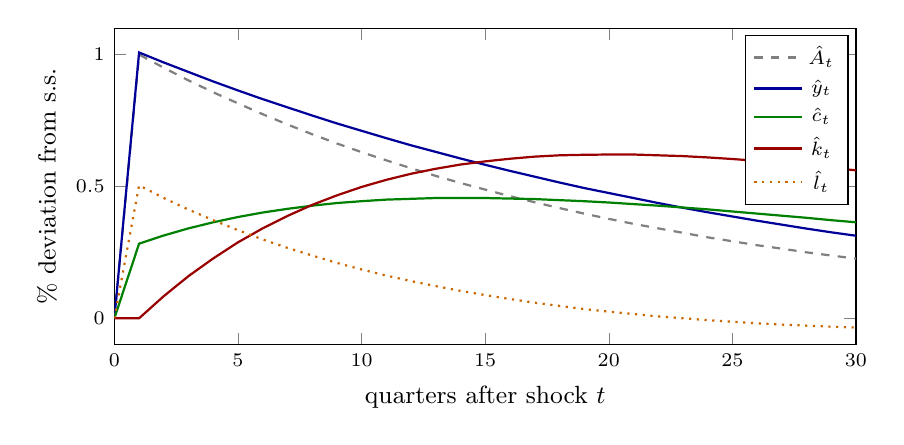
\begin{tikzpicture}
\begin{axis}[width=11cm,height=5.6cm,xmin=0,xmax=30,ymin=-0.1,ymax=1.1,
  xlabel={quarters after shock $t$},ylabel={\% deviation from s.s.},
  legend style={font=\scriptsize,at={(0.99,0.98)},anchor=north east},
  tick label style={font=\scriptsize},label style={font=\small}]
\addplot[thick,gray,dashed] coordinates {(0,0.000) (1,1.000) (2,0.950) (3,0.902) (4,0.857) (5,0.815) (6,0.774) (7,0.735) (8,0.698) (9,0.663) (10,0.630) (11,0.599) (12,0.569) (13,0.540) (14,0.513) (15,0.488) (16,0.463) (17,0.440) (18,0.418) (19,0.397) (20,0.377) (21,0.358) (22,0.341) (23,0.324) (24,0.307) (25,0.292) (26,0.277) (27,0.264) (28,0.250) (29,0.238) (30,0.226)};
\addlegendentry{$\hat A_t$}
\addplot[thick,blue!60!black] coordinates {(0,0.000) (1,1.008) (2,0.970) (3,0.934) (4,0.898) (5,0.864) (6,0.831) (7,0.800) (8,0.769) (9,0.739) (10,0.711) (11,0.683) (12,0.656) (13,0.631) (14,0.606) (15,0.582) (16,0.559) (17,0.537) (18,0.515) (19,0.494) (20,0.475) (21,0.456) (22,0.437) (23,0.419) (24,0.402) (25,0.386) (26,0.370) (27,0.355) (28,0.340) (29,0.326) (30,0.313)};
\addlegendentry{$\hat y_t$}
\addplot[thick,green!50!black] coordinates {(0,0.000) (1,0.283) (2,0.314) (3,0.341) (4,0.364) (5,0.384) (6,0.401) (7,0.415) (8,0.427) (9,0.437) (10,0.444) (11,0.450) (12,0.453) (13,0.456) (14,0.456) (15,0.456) (16,0.454) (17,0.452) (18,0.448) (19,0.444) (20,0.439) (21,0.433) (22,0.427) (23,0.420) (24,0.413) (25,0.405) (26,0.397) (27,0.389) (28,0.381) (29,0.372) (30,0.364)};
\addlegendentry{$\hat c_t$}
\addplot[thick,red!60!black] coordinates {(0,0.000) (1,0.000) (2,0.084) (3,0.160) (4,0.227) (5,0.288) (6,0.341) (7,0.388) (8,0.430) (9,0.466) (10,0.498) (11,0.525) (12,0.548) (13,0.567) (14,0.583) (15,0.595) (16,0.605) (17,0.613) (18,0.618) (19,0.620) (20,0.621) (21,0.621) (22,0.618) (23,0.615) (24,0.610) (25,0.604) (26,0.597) (27,0.589) (28,0.580) (29,0.571) (30,0.561)};
\addlegendentry{$\hat k_t$}
\addplot[thick,orange!80!black,dotted] coordinates {(0,0.000) (1,0.504) (2,0.456) (3,0.412) (4,0.372) (5,0.334) (6,0.299) (7,0.267) (8,0.238) (9,0.210) (10,0.185) (11,0.162) (12,0.141) (13,0.122) (14,0.104) (15,0.088) (16,0.073) (17,0.059) (18,0.047) (19,0.035) (20,0.025) (21,0.016) (22,0.007) (23,-0.000) (24,-0.007) (25,-0.013) (26,-0.019) (27,-0.024) (28,-0.028) (29,-0.032) (30,-0.035)};
\addlegendentry{$\hat l_t$}
\end{axis}
\end{tikzpicture}
\end{center}
How to read the figure: it plots the IRFs to a 1\% TFP shock at $t=1$, computed from the policy rules with the example parameters above. The horizontal axis is quarters after the shock; the vertical axis is the percent deviation from steady state. Output and hours jump on impact (output by more than TFP because hours rise); consumption rises by less and keeps rising (households smooth consumption, saving much of the windfall); capital is predetermined, so it starts at 0 and builds up slowly, peaking long after the shock. Because the extra capital wears off only slowly, output stays above steady state for many periods: the ``long tail'' of the general case.

%=====================================================================
\subsection{Frisch elasticity of labour supply \pg{67}}

\paragraph{Definition.} The \textbf{Frisch elasticity} is the elasticity of hours with respect to the wage, holding the marginal utility of wealth $\lambda_t$ (here $\lambda_t=1/c_t$) fixed:
\[
\varepsilon^{F}\equiv\frac{\partial\ln l_t}{\partial\ln w_t}\Big|_{\lambda_t\text{ fixed}}.
\]
Holding $\lambda_t$ fixed shuts down the income (wealth) effect, so the Frisch elasticity measures the pure \emph{intertemporal substitution} of labour: how willingly people shift work toward periods with temporarily high wages. Since temporary shocks barely change lifetime wealth, this is the elasticity that matters for business-cycle fluctuations in hours.

\paragraph{Case 1: separable power disutility.} Let $u=\ln c-\chi\frac{l^{1+\gamma}}{1+\gamma}$ with $\chi,\gamma>0$. The $[l_t]$ FOC (as in the Lagrangian above) is
\begin{align*}
\chi l_t^{\gamma}&=w_t\lambda_t\\
\text{Take logs:}\quad \ln\chi+\gamma\ln l_t&=\ln w_t+\ln\lambda_t\\
\text{Differentiate with }\lambda_t\text{ fixed:}\quad \gamma\,d\ln l_t&=d\ln w_t\\
\Rightarrow\quad \varepsilon^F&=\frac1\gamma .
\end{align*}

\paragraph{Case 2: the log-leisure utility of this section.} With $u=\ln c+b\ln(1-l)$ the FOC is $\frac{b}{1-l_t}=w_t\lambda_t$.
\begin{align*}
\text{Take logs:}\quad \ln b-\ln(1-l_t)&=\ln w_t+\ln\lambda_t\\
\text{Differentiate with }\lambda_t\text{ fixed:}\quad \frac{dl_t}{1-l_t}&=d\ln w_t\\
\text{Use }dl_t=l_t\,d\ln l_t:\quad \frac{l_t}{1-l_t}\,d\ln l_t&=d\ln w_t\\
\Rightarrow\quad \varepsilon^F&=\frac{1-l^*}{l^*}\quad\text{(evaluated at steady state)}.
\end{align*}
\begin{keybox}[title=Frisch elasticity]
\[
u=\ln c-\chi\tfrac{l^{1+\gamma}}{1+\gamma}:\ \ \varepsilon^F=\frac1\gamma;\qquad\qquad
u=\ln c+b\ln(1-l):\ \ \varepsilon^F=\frac{1-l^*}{l^*}\ \ (l^*=\tfrac13\Rightarrow\varepsilon^F=2).
\]
\end{keybox}
Interpretation: in the log-linear labour condition \eqref{eq:s6_L4}, the coefficient on $\hat l_t$ on the right is $\frac{l^*}{1-l^*}=1/\varepsilon^F$. A larger Frisch elasticity makes hours respond more strongly to wage movements, which helps the RBC model generate realistic fluctuations in hours. Micro estimates are usually much smaller (around $0.5$ or less), a well-known tension for the model.
